\documentclass[twocolumn]{article}
% {amsart}
\usepackage[top=0.75in, left=0.65in, right=0.65in, bottom=0.6in]{geometry}

\usepackage{float}

% \usepackage{url}
% \usepackage{xurl}
\usepackage[pdftex]{hyperref}

%\usepackage{code}
\usepackage{listings}
% \usepackage{cite}
\usepackage{latexsym}
\usepackage{amsmath}
\usepackage{amssymb}
\usepackage{graphicx}
% IPA symbols. safe turns off overrides for like \! which I still want
\usepackage[safe]{tipa}
\usepackage{chessboard}
\usepackage{supertabular}
\usepackage{enumitem}

\usepackage[most]{tcolorbox}

% lets me explicitly set a. or 1. etc. as enum label
% \usepackage{enumitem}

\pagestyle{empty}

\usepackage{ulem}
% go back to italics for emphasis, though
\normalem

% do "fancy" stuff like verbatim in footnotes
\usepackage{fancyvrb}
\VerbatimFootnotes

\usepackage{natbib}

\interfootnotelinepenalty=0
\setlength{\footnotesep}{2em}


% Style for code listings.
\lstdefinestyle{codestyle}{
  basicstyle=\ttfamily\footnotesize,
  breaklines=false,
  keepspaces=true,
}

\lstset{style=codestyle}

\newcommand\sfrac[2]{\!{}\,^{#1}\!/{}\!_{#2}}

\newcommand\tetrispiece[1]{\,\includegraphics[height=0.8em]{#1}\hspace{0.1em}}
\newcommand\ivert{\tetrispiece{i_vert}}
\newcommand\ihoriz{\tetrispiece{i_horiz}}
\newcommand\squarepiece{\tetrispiece{square}}

\newcommand\tup{\tetrispiece{t_up}}
\newcommand\tdown{\tetrispiece{t_down}}
\newcommand\tleft{\tetrispiece{t_left}}
\newcommand\tright{\tetrispiece{t_right}}

\newcommand\jup{\tetrispiece{j_up}}
\newcommand\jleft{\tetrispiece{j_left}}
\newcommand\jdown{\tetrispiece{j_down}}
\newcommand\jright{\tetrispiece{j_right}}

\newcommand\zhoriz{\tetrispiece{z_horiz}}
\newcommand\zvert{\tetrispiece{z_vert}}

\newcommand\shoriz{\tetrispiece{s_horiz}}
\newcommand\svert{\tetrispiece{s_vert}}

\newcommand\lup{\tetrispiece{l_up}}
\newcommand\lleft{\tetrispiece{l_left}}
\newcommand\ldown{\tetrispiece{l_down}}
\newcommand\lright{\tetrispiece{l_right}}


% XXX the collection of crap above causes a first page
% with just "1" on it (probably conflicting packages). This
% magic just drops the first page, which is of course not
% the right solution, but...
\usepackage{atbegshi}% http://ctan.org/pkg/atbegshi
\AtBeginDocument{\AtBeginShipoutNext{\AtBeginShipoutDiscard}}

\begin{document}

\title{Harder Drive: Hard drives we didn't want or need}
\author{Dr.~Tom~Murphy~VII~Ph.D.}\thanks{
Copyright \copyright\ 2022 the Regents of the Wikiplia Foundation.
Appears in SIGBOVIK~2022 with the
Input/Output error of the Association for Computational Heresy; {\em IEEEEEE!}
press, Verlag-Verlag volume no.~0x40-2A. 6.6e-11 $N m^2kg^{-2}$
}

\renewcommand\th{\ensuremath{{}^{\textrm{th}}}}
\newcommand\st{\ensuremath{{}^{\textrm{st}}}}
\newcommand\rd{\ensuremath{{}^{\textrm{rd}}}}
\newcommand\nd{\ensuremath{{}^{\textrm{nd}}}}

\renewcommand\paragraph[1]{\smallskip \noindent{\bf #1}\enspace}

\date{7 April 2022}

\maketitle \thispagestyle{empty}

\sloppypar


\section{Introduction}

\subsection{Chainsaws}

At first glance, it seems that the maximum number of chainsaws that a
person can wield is two: One per hand. This is known as {\em
  dual-wield}. It may be possible to achieve more using
``one-man-band'' arrangements (shin- and knee-wielded chainsaws, elbow
saws, a mouth-held chainsaw activated by blowing into it like a
harmonica) but a more natural way to scale is by juggling the saws
into the air. Now at second blush it seems that an arbitrary number of
saws can be simultaneously equipped, by simply throwing the chanisaws
higher into the air. This configuration is known as $\infty$-wield.
However, throwing chainsaws higher and higher eventually reaches
physical limits. Once the thrown saws reach the escape velocity of
11.186$\sfrac{km}{s}$, they will not fall back to Earth, and can
hardly be considered brandished by the juggler. Ignoring air resistance
(the chainsaws cut through the air like butter), these saws can be
% FIXME this is probably wrong, since these formulas would keep giving
% larger and larger heights (not infinity) past the escape speed.
% simulate?
thrown to a maximum height of $\sfrac{11,186^{2}}{2 \times 9.8} = 6,384 km$,
taking $\sfrac{2 \times 11,186}{9.8} = 2,282 s$ for the round trip.

% Note! escape velocity does not depend on direction!

This loop has two problems: First, it is not the longest possible airtime.
Second, it can only be used for one chainsaw at a time, as the saws will
otherwise interfere with one another along the out-and-back path.
Instead we can juggle the saws into orbits

Johann Sebastian Kepler's third law:
$$T = 2 \pi \sqrt{\frac{a^3}{GM}}$$

$a$ is the semi-major axis (largest radius) of the ellipse (the orbit time
does not depend on the eccentricity!), $G$ is the gravitational constant,
and $M$ is the mass of Earth. Note that this period is arbitrarily large
if we can achieve a larger semi-major axis, but at a certain point (when
we reach the escape speed) the orbit ceases to be an ellipse and we never
get the chainsaw back.

120731001 time steps is 1207310.01 seconds, 335.36 hours.


Upon a third look, we need not throw the chainsaws straight upward.
https://en.wikipedia.org/wiki/Orbital\_period

Overall, the important lesson here is creativity with dimensional
analysis: We can achieve a quantity of {\it chainsaws} by multiplying
some {\it chainsaws per second} by some {\it seconds}.

\subsection{Juggling with data}

Now imagine that instead of chainsaws, we are juggling something more
dangerous: Data.

One potential setup would be a powerful directional antenna, which
broadcasts a stream of data towards the horizon. For radio waves below
40 MHz, significant reflections off the ionosphere occur, bouncing the
waves back to Earth. They may also reflect off the ground, and again
off the ionosophere, and in principle make their way fully around the
planet. The antenna is paired with a receiver in the same location,
which accepts the signal and retransmits it, ``juggling'' it back into
circulation.
% XXX Figure

Since a full trip around the Earth is 40,000 km (and significantly
more in this setup due to reflections) and radio waves take time to
propagate, this orbit takes at least 150ms to
% XXX should it be 20 because of Nyquist?
complete. As a result, we can have 0.15 sec $\times$ 40,000,000
bits/sec = 750 kilobytes of data outstanding in the steady state. When
data we are interested reaches the receiver we can ``read'' it, and of
course we can choose to retransmit modified data to perform a
``write,'' This is similar to the rotation of a hard drive, with the
fixed read/write head waiting for the ``orbiting'' platter.

This author does not have sufficient skill to construct a system,
which would probably not work in practice anyway---the reflections
probably do not make it all the way around the Earth, and the noise
from other radio waves would offer significant interference.

A superior arrangement would place repeater towers along the great
circle. This would clearly work but would require an investment
in real estate throughout the world.

The main reason not to do this is that 750kb is a trivial amount
of storage; a similar magnitude is found incidentally in disposable
consumer devices (Section~\ref{sec:cue}).


Of course, if we are retransmitting the signal anyway, we do not need
to send it in the same direction. It is much simpler to send it
directly back, like an echo.

\subsection{ICMP Echo}

Back when the internet was a collaborative and basically nice place,
the Internet Control Message Protocol (ICMP) was proposed as a way for
network nodes to help each other out. This protocol allows sending
messages like ``hey this address is down!'' or other tips. Since it is
easy to forge ICMP messages, most off these have potential for abuse
(like telling you the site you're talking to is down) and are no
longer commonly honored. (As another indicator of the era, these
internet standards are known as ``Requests for Comment'', with ICMP
described in RFC 792~\cite{rfc792}. On the modern internet we still
have requests for Comment, but they are almost universally accompanied
by requests for Like and Subscribe.)

\newcommand\icmpecho{{\tt ECHO}}
\newcommand\icmpechoreply{{\tt ECHO REPLY}}

However, many hosts will still respond to an \icmpecho\ packet with
\icmpechoreply.
This is typically used to ``ping'' a host: The source sends
\icmpecho\ to the destination with some identifying information and an
embedded timestamp; the destination sends \icmpechoreply\ with that
same data back to the source, and the source can calculate the
round-trip time.

Since there are hosts throughout the world that will already reply to
\icmpecho\ messages, this could be a perfect setup for juggling data!
The {\tt data} field of the \icmpecho\ can store the bytes of interest.
When we receive an \icmpechoreply\ we will ``read'' or ``write'' that
data if needed, and then immediately broadcast another \icmpecho.
Since we do not retain the data otherwise, it will be stored
``inside'' the internet itself: Inside the buffers of routers but also
as moving photons inside fiber optics, flowing charge in ethernet
cables, and so on.

In principle we should be able to saturate our internet connection
with outgoing \icmpecho\ and incoming \icmpechoreply; even on a
consumer plan (these days on the order of 1 gigabit/sec) we may be
able to store significant amounts of data. If we ping a host on the
Earth's antipode, the round trip time will be at least 150ms (speed of
light and circumference are limits here as well). $1 Gb/sec$ $\times$
$0.15 sec$ = 833 Megabytes.

In practice this proves to be much more difficult. Alas, even the
apparently harmless \icmpecho\ has been regularly abused for
denial-of-service attacks, such as the ``Ping of
Death''\cite{wikipediapingofdeath} and ``Smurf
attack''\cite{wikipediasmurfattack}. Thus, hosts almost always have
hard limits that we have to work within. We will face the following
difficulties that cause us to fall far short of the ideal above:

\begin{enumerate}
\item Hosts limit the size of an \icmpecho\ packet they will respond to.
  512 bytes of payload is a typical limit for a fairly permissive
  host,\!\footnote{
    Allegedly, ``all hosts are required to be able to reassemble datagrams of
    size up to 576 bytes,''\cite{XXX} but I guess most do not care about this
    or consider it better than dropping all pings. There are not many
    legitimate uses for a payload of this size, anyway.
  }
  %
  but many will reject payloads more than a few dozen bytes. The IP
  header (20 bytes) and ICMP header (8 bytes) thus contribute significant
  overhead.

\item Hosts have global limits on the rate of incoming and outgoing ICMP
  messages.
\item Consumer internet connections have built-in throttling of ICMP
  messages, perhaps to limit the impact of Denial-of-Service attacks
  originating from their networks.
\item Pings are ``best effort'' and readily dropped by congested
  routers without retries (this can even be a desirable property for
  measuring network congestion).
\end{enumerate}

\subsection{Pinging the internet} \label{sec:ping-internet}

While developing code that can process many thousands of pings per second
and investigating these limitations, I figured I might as well ping the
entire internet.

Here by internet I mean ``IPv4 address space.'' I don't care about
IPv6 which has {\it way too many addresses} (plus like, call me when
you are at least version 7, right?). There are only $2^{32}$ IPv4
addresses, which is no longer that big of a number. I wrote a fairly
simple program {\tt pingy.exe} which pings all of the hosts of the
form {\tt *.*.c.*} for some ${\tt c} \in \{0,\ldots,255\}$ in a random
order. For each one it saves the number of milliseconds of round-trip
time (or records special sentinel values for ``timeout'' or ``wrong
data returned'') in a single byte. This results in 256 files, which
assembled are 4.2 Gigabytes.

This turned out to be much more logistically challenging than I
expected. Na\"ively I should be able to send millions of pings per
second, but the packets are dropped somewhere if I exceed about 1000
pings/sec. Even at 1000 pings/sec (a trivial amount of bandwidth) this
behavior seems to wreak havoc on my home network; other devices
sharing the connection get extremely bad performance, a no-no for the
Work-from-Home video call life of the pandemic. This could be because
my internet provider throttles ICMP; it could also be that some
hardware or software in the path is not able to handle thousands of
different IP addresses each second (e.g. there may be fixed-size NAT
tables). I tried using a VPN, but this had a much lower success rate;
the VPN egress point probably throttles ICMP to prevent DDoS attacks,
and it's possible that many internet gateways also simply block ICMP
from known VPN endpoints since they are obvious choices for people up
to no good. Anyway, what I thought might take a few hours or a weekend
ended up taking months. Eventually I rented time on several machines
in different data centers to parallelize the process; this also
produced a higher ping response rate than my home network, so I redid
all of the already-completed sections for uniformity. The results make
a nice poster, though and are in Figure~\ref{fig:internet}.

\begin{figure*}[tp]
\includegraphics[width=\textwidth]{internet}
\caption{ The results of pinging all $2^{32}$ IPv4 addresses in early
  2022. The IP addresses are plotted along a 16-level Hilbert
  Curve\cite{hilbert1891ueber}. The full image is 65536 $\times$ 65536
  pixels (and 4.2 Gigabits), which alas cannot be fit within the
  preposterously limited SIGBOVIK page and PDF size guidelines. This
  image is 2048 $\times$ 2048, so each pixel represents $32 \times 32$
  hosts, with the level of grey giving the response rate (white = no
  response). There are several obvious patterns, which can be
  cross-referenced with Figure~\ref{fig:internetlegend} to see the
  first octet of the IP address. Some interesting regions: There are
  almost no responses in the top-right region, which is {\tt 224.*} to
  {\tt 255.*}; these are the former ``Class~D'' and ``Class~E''
  segments which are {\it multicast} and {\it reserved} respectively.
  There is a dark block at the center that almost always receives
  responses, which is from the {\tt 127.*} ``loopback'' address. This
  all makes sense. It is interesting to see how active regions allocate
  their space; some have a variety of distinct patterns and others
  seem uniformly random.
%
  This way of plotting the address space is basically canonical, so it
  is a bit disappointing not to find any graphical messages. Like,
  how cool would it be to embed a micro QR code in some 16x16 subnet
  that says {\tt IPv6sux}? It would be a little bit cool, is how cool.
} \label{fig:internet}
\end{figure*}

\begin{figure*}[htp]
  \includegraphics[width=2in]{legend}
  \caption{ XXX } \label{fig:internetlegend}
\end{figure*}

9.18\% of addresses responded successfully within 4 seconds. Only
4,529 hosts (0.000105\%) replied with the wrong data.

\subsection{Harder Drive: Pingu}

I then built a block device, called {\tt pingu}\footnote{Named for the
  classic stop-motion penguin of the same name. Also as in ``i ping u
  2 store data\,\, thx 4 ur help''} using this concept. The smallest
drive that can be formatted and mounted on linux is 51,200 bytes,
using the FAT12 filesystem common on DOS floppy disks in the
1980s.\cite{wikipediafat12}\footnote{ Try: \verb+mkfs.vfat -F 12 -v -a -n "PINGU"+ } So
the device consists of one hundred 512-byte blocks. Each block will
be stored inside multiple outstanding pings (for redundancy) with
a 512-byte payload.

Despite pinging the whole internet in Section~\ref{sec:ping-internet},
we use a fixed set of IP addresses here. The reason for this is that
we want a set of IP addresses that are stable, reliable, and have high
latency. They must respond to pings with a 512-byte payload. We would
also prefer these to have uncorrelated failures, because if all of the
outstanding pings fail for a block, then the data is permanently lost.
So we want them to be geographically diverse, for example. I also
prefer to use major commercial sites that can clearly bear the load,
as opposed to e.g. someone's cell phone (who may even have metered
bandwidth). I produced the list of ~75 hosts by searching for ``most
popular websites in Madagascar'' (etc.) and manually pinging them to
make sure the criteria are met, particularly the latency. Many sites
worldwide use content networks (or are simply hosted in the United
States) and so they are much faster than the speed of light would
suggest. I found that databased-backed sites (like e-commerce pages)
were less likely to be on content networks than e.g.~news sites, which
makes sense.

Implementing this block device is tricky: We can only process a read
or write at the moment a ping returns from the network.

\paragraph{Blocks.} Each block contains a sequence and version counter,
as well as the set of outstanding pings (send time and host IP, so that
we can detect timeouts and update host stats). There is also a queue
of pending reads and writes. The contents of the block is not stored.

\paragraph{Reading.} A call to read a block inserts itself in a queue
and then blocks on a condition variable; it will not return until we
receive a ping that belongs to that block.

\paragraph{Writing.} A call to write is accompanied by some data (the
caller has allocated it). These are also enqueued and block until
we receive a ping from the host and can process it. In the general
case we cannot process a write without receiving the ping, because
the write may only be to a portion of the block (and so we need to
know the data outside that region). When we process the write we
update the version counter so that we don't later use the data
from any other outstanding redundant pings.

\paragraph{Hosts.} With each host (IP address) we also keep track of
its recent latency and reliability (exponentially-weighted moving
averages) as well as a token bucket to prevent exceeding a prescribed
number of pings per second to that host.

\paragraph{Processing.} A single thread calls {\tt select} to see
if the socket is ready. For juggling we need to simultaneously be
ready for both {\em reading} and {\em writing}. We then read a ping,
and use its sequence number to route it to the correct block. The
block validates the ping (if it has the wrong version it's just
discarded, for example) and uses it to fulfill any outstanding reads
(copying into their buffers and notifying the condition variable so
those calls can return). We then process any writes to compute the
updated data, and juggle the data back onto the network by sending
pings until we are at the target redundancy (there will be at least
one, since we just received one of the outstanding pings).

\paragraph{Initialization.} The loop just described is driven by
the receipt of pings, so we also need to kick off the process by
sending initial pings for each block. After each call to select
we initialize a single block if it has not yet been, and has at
least one outstanding write.

\paragraph{Visualization.} The block device runs in userspace,
but not in a way that supports a UI. To view the device while it's
being used, I send text status updates to {\tt nbdkit}'s debugging
interface, and then pipe these to an SDL-based visualization. It show
the status of each block and statistics on each host, as well as
read/write activity. It is fun to watch the process of formatting
it for FAT12 and reading/writing files.

\subsubsection{Results.}

Benchmarking approach.

What file to store.



\section{Tetris, the Soviet Mind Game} \label{sec:tetru}

Sorry to remind you about Russia's illegal attack on Ukraine, but

The characters of Tetris are:

ivert: \ivert
ihoriz: \ihoriz
squarepiece: \squarepiece

tup: \tup
tdown: \tdown
tleft: \tleft
tright: \tright

jup: \jup
jleft: \jleft
jdown: \jdown
jright: \jright

zhoriz: \zhoriz
zvert: \zvert

shoriz: \shoriz
svert: \svert

lup: \lup
lleft: \lleft
ldown: \ldown
lright: \lright


A Tetris board is 10 columns wide and 20 rows high. Even if we could
use every one to store a bit, 200 bits is far too few to create a
filesystem. Therefore we'll use an array (or if you will, a {\em
  Beowulf cluster}) of Tetris games to create the block device.

We will store a bit pattern in a Tetris game by playing a series of
moves to create a specific pattern in the playfield. We can then read
the data directly from that pattern. If we need to write a new
pattern, we reset the game and begin again.

Each ``line'' of the playfield has 10 positions, each of which could
have a block in it or not, so we could consider storing 10 bits.
However, due to the rules of Tetris, if all of the cells are filled,
then the line is cleared. This would make it impossible to store the
pattern {\tt 1111111111}. It will also be impossible to store the
pattern of all zeroes, because an empty line cannot support any pieces
above it, so empty lines can only appear in some completely-empty
prefix of the playfield. Additionally, observe that a Tetris board
always has an even number of cells filled. We can only add 4 blocks
by dropping a piece, or remove 10 blocks by clearing a line, which
can only yield even numbers. So it will also benefit us to use
one cell per line for parity. This leaves 8 cells per line, encoding
a single byte, which is a nice round number.

We can't use the full height of the playfield, since we need some
room in which to maneuver pieces. 8 is a convenient choice here as
well (although more is possible). Each Tetris game will store 64 bits
in eight lines, each with eight bits.
% I tested 10 bits; 529 examples successful. 12 fails, though (would
% perhaps need to plan inside a more cramped space? or is the game
% just getting too fast and we can't force RNG?)

\subsection{Playing Tetris}

Now the problem is: Given a blank board, what sequence of moves do
we make in order to produce the target pattern?

This is not easy. To begin with, Tetris normally gives the player
pieces at random. As anyone who plays Tetris knows, it can be very
disruptive to your strategy when you don't get the piece you need for
some time. The first step will be to reverse engineer the pseudorandom
piece drop logic so that we can influence the sequence of pieces that
are dropped.

\subsubsection{Random pieces}

The core of the piece drop logic is a 16-bit linear feedback shift
register~\cite{golomb1967shift}\footnote{Fittingly, Golomb was a
  pioneer in both shift registers {\em and} polyominoes, the latter
  which influenced Tetris itself!}. Equivalent C code is given in
Figure~\ref{fig:nextrng}. This 16-bit state is updated on every frame
(and sometimes more; see below), and has period 32767.\footnote{ It is
  possible to create a 16-bit LFSR with a period of 65535, but this
  one is simply deficient. This is one of several small problems with
  the code. I hope to one day release a ``hot fix'' ROM that fixes
  this and other bugs and inefficiencies.}

\begin{figure}
  \begin{lstlisting}[language=C]
uint16_t NextRNG(uint16_t state) {
  uint16_t carry = ((state >> 9) ^ (state >> 1)) & 1;
  return (state >> 1) | (carry << 15);
}
  \end{lstlisting}
  \caption { The simplified code for Tetris's pseudorandom number
    generator, which resides at address {\tt 0xAB47} in the Tetris
    code. This is a 16-bit two-tap LFSR: The {\tt carry} is the
    exclusive-or of the second and tenth least significant bits. We
    right-shift off the least significant bit and use the carry as the
    new most-significant bit.} \label{fig:nextrng}
\end{figure}

The pseudorandom state is extended with two additional bytes: One
giving the last dropped piece (a piece is ``dropped'' into a queue so
this is actually the ``next piece'' to the player) and the count of
pieces dropped (mod 256). When the player places a piece, the routine
at address {\tt 0x9907} uses the LFSR state and these two bytes to
drop a new piece (and update the state):

\begin{lstlisting}[language=C]
RNGState NextPiece(RNGState s) {
  constexpr std::array<uint8_t, 8> PIECES = {
    0x02, 0x07, 0x08, 0x0A, 0x0B, 0x0E, 0x12,
    // not used
    0x02,
  };

  s.drop_count++;

  uint8_t a = (s.lfsr_hi + s.drop_count) & 7;

  if (a == 7 || PIECES[a] == s.last_drop) {
    // re-roll if out of bounds, or repeat
    s = NextRNG(s);
    // mod 7 forces in-bounds, but allows repeats
    a = ((s.lfsr_hi & 7) + s.last_drop) % 7;
  }
  
  s.last_drop = PIECES[a];
  return s;
}
\end{lstlisting}

It uses three bits of the RNG state to pick a random piece (there are
7 different shapes, and the game always drops a shape in the same
orientation). If it rolls an 8, or if the selected piece is the same
as the last one, then it re-rolls: Another update of the LFSR, and
then a different weird procedure to pick the piece index. Here the
result is {\sf mod}~7, so it is always in bounds. The code only
re-rolls once, so it is possible to drop the same piece twice in
a row, just less unlikely.

Ideally we would be able to select a sequence of pieces that we want,
and then force Tetris to give us those pieces. Since the LFSR update
runs every frame, we can use a different number of frames while
placing a piece, and get a different LFSR state at the point {\tt
  NextPiece} is called. The LFSR is ``pretty good,'' so we
can easily cause the first roll to be whatever value we want by
just waiting. In the worst possible case we need to pause 98 frames
before seeing all 8 rolls (Figure~\ref{fig:rollhisto}), which is
1.5 seconds at the NES frame rate.

\begin{figure}
  \includegraphics[width=\linewidth]{rollhisto}
  \caption {
    XXX caption me
    } \label{fig:rollhisto}
\end{figure}

However, this does not work for re-rolls, which is the only way to get
the same piece twice in a row. Even though we use the same ``pretty
good'' LFSR, two successive calls are highly correlated. There are
only two possible new values for the high byte of the LFSR
(\verb|s.lfsr_hi|): \verb|(s.lfsr_hi >> 1)| and \verb|128 + (s.lfsr_hi >> 1)|.
Worse, since these are congruent modulo $8$, we really just have
\verb|(s.lfsr_hi >> 1)|.
 
As a result, even if you have complete control over the LFSR state
(but not the previous piece nor drop count), there are a limited
number of outcomes possible from the reroll. We can just inspect all
the possible combinations of previous piece and drop count to see that
with some there are at most 4 possible rerolls, and as few as 2. For
example, if the previous piece is \shoriz\ and 253 pieces have been
dropped so far, then only \tup, \shoriz, and \jdown\ can result. So
here it is possible to get two \shoriz\ pieces in a row. But if the
last piece was \ihoriz, and 3 pieces have been dropped so far, then
only \zhoriz\ and \lup\ are possible from a re-roll. Since
\ihoriz\ cannot result from the first roll and is not possible for the
re-roll in this state, it is impossible to get two \ihoriz\ pieces in
a row on the 3\rd\ and 4\th\ drop. All pieces other than
\squarepiece\ periodically have this problem.\!\footnote{This is
  another example of a deficiency in the code that could easily be
  fixed. If we simply remove the instruction at {\tt 0x9925},
  \verb+AND #$07+ (so that the re-roll just uses
  \verb|(s.lfsr_hi + s.last_drop) % 7|) then {\it all} configurations
  can now produce all pieces upon re-roll. The modulus is computed
  with a loop, so this is not a strict efficiency improvement, but
  efficient alternatives exist, like \verb|((s.rng2 & 15) ^ s.last_drop) % 7|.
} Even when it is possible, it may
require a long drought to get the LFSR in a rare working state.

By manipulating the RNG we will be able to achieve any sequence of
pieces, except if that sequence contains repeats. There is a similar
consideration for the first two pieces of the game, which are
generated on the same frame (current and next piece) and so only
certain combinations are possible. To simplify this issue
away, we begin by always playing the same starting sequence:
\squarepiece 0 \lleft 3 \jright 6 \lright 2 \jleft 7. This means to
drop a \squarepiece\ in column 0 (the leftmost column), \lleft\ in
column 3 (the left edge of the piece goes in column 3), etc. This
sequence clears two lines, leaving the board empty, with the only
constraint now being that we cannot start with a \jleft\ piece.

\subsubsection{Planning}

With a smart algorithm, it would be possible to plan moves within
these constraints to generate moves for any byte pattern that we want
to create. However, this is not an easy feat. Creating very sparse
patterns (few {\tt 1} bits) is pretty challenging because pieces can
only be placed on top of existing blocks (Figure~\ref{fig:tetrisdot}).

\begin{figure}
  \includegraphics[width=\linewidth]{tetrisdot}
  \caption{
    A screenshot of NES Tetris after playing for 2 minutes and 46
    seconds, encoding the sequence {\tt 0, 0, 0, 0, 64, 0, 0, 0}.
    Floating blocks like this are very difficult to create. Try
    creating a position like this, even by selecting your favorite
    piece at each step!
  } \label{fig:tetrisdot}
\end{figure}

Instead, the approach I took was to build a modular solution for each
byte. We always place the board in a standard configuration
(Figure~\ref{fig:encodingscheme}) where a \svert\ piece is in column
0. A portion of the board below it contains the encoded bytes (one per
row) and parity (first two columns). We do not depend on the contents
of this portion at all, so the first moves must hang off of the
\svert\ piece. For each byte, we need to come up with a series of
moves that takes a starting configuration like this, encodes the byte
(and its parity) in the bottom row, and then recreates the starting
configuration with the \svert\ piece moved up one line. These plans
are also nontrivial to construct, but we can take our time to solve
each byte offline. Then, because they are compositional, we can assemble
them to create any sequence of bytes at runtime.

\begin{figure}
  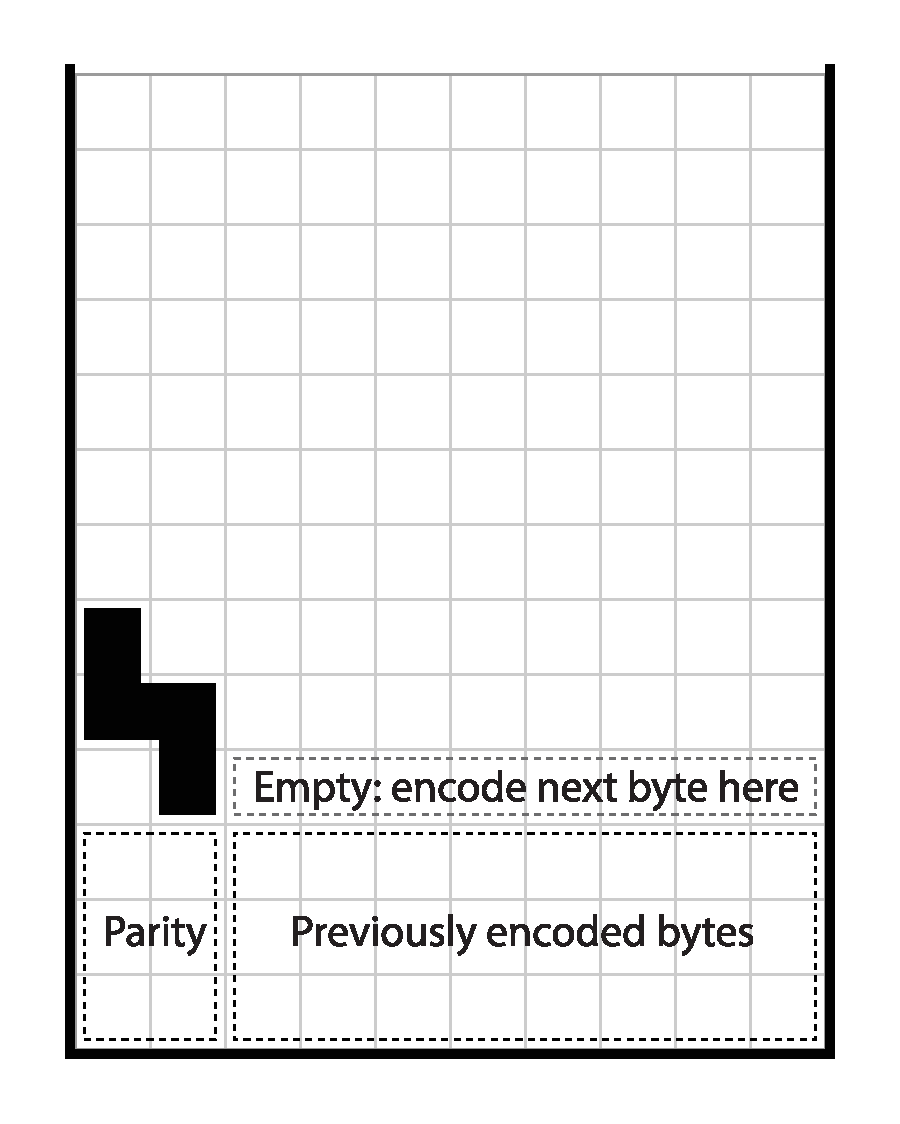
\includegraphics[width=\linewidth]{encodingscheme}
  \caption{
    The start state as we encode each byte. The \svert\ piece in the
    left column is known to be present, but we do not know the state
    of any blocks below it. We will build off this ... XXX
    } \label{fig:encodingscheme}
\end{figure}

\begin{figure}
  \begin{tabular}{cc}
  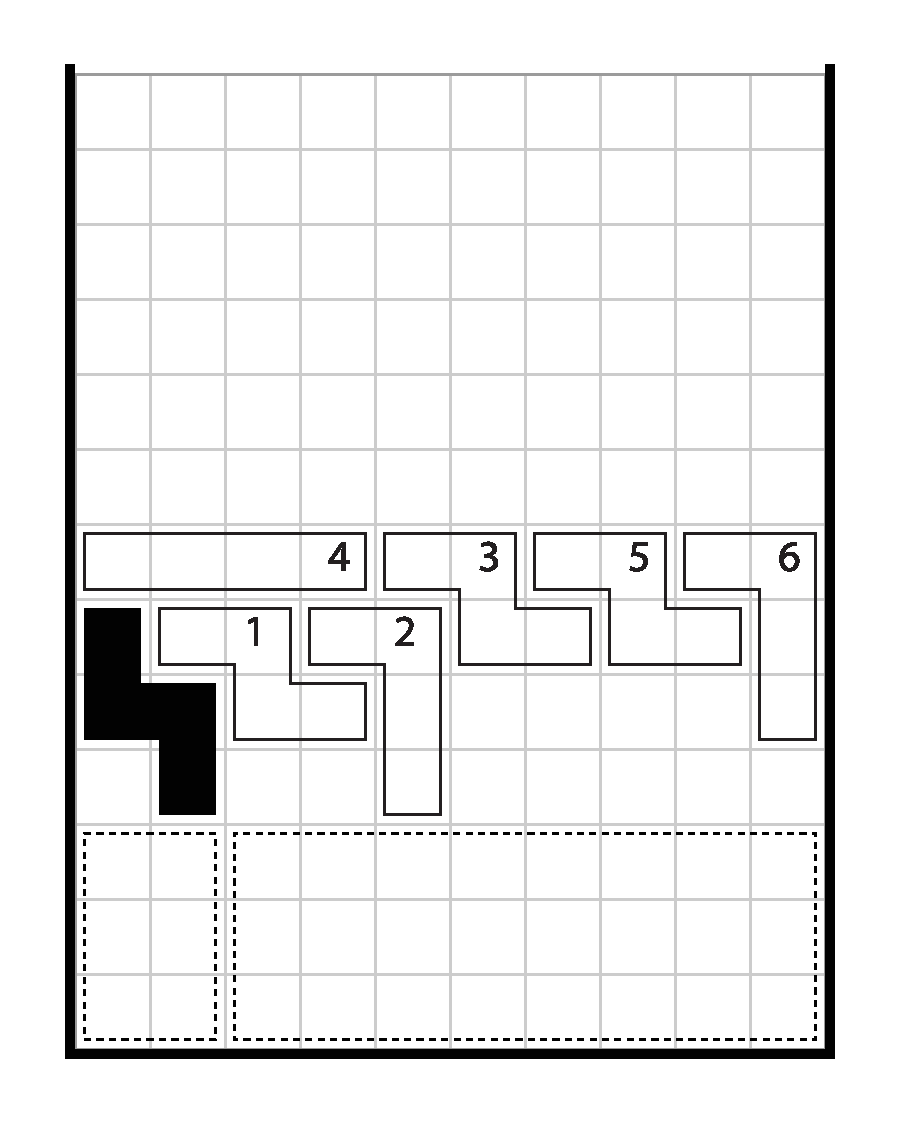
\includegraphics[width=0.4 \linewidth]{encode26a} &
  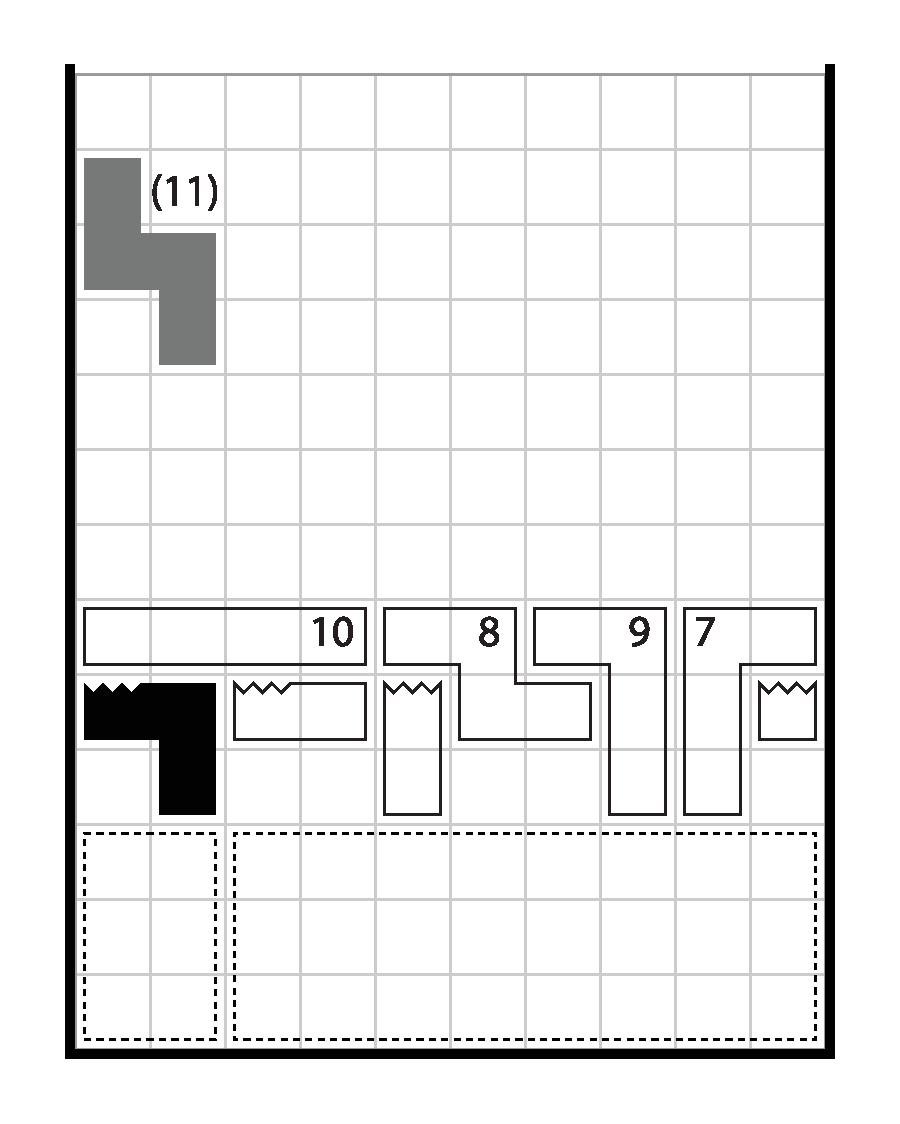
\includegraphics[width=0.4 \linewidth]{encode26b} \\
  (a) & (b)
  \end{tabular}
  \caption{ Encoding {\tt 0x26}, which is {\tt 0b0011010}. This is one
    of the easiest bytes. In (a), drops 1--6 build off of the starting
    \svert, conveniently dropping a {\tt 1} bit in column 4 along the
    way. These moves clear the two top lines, leaving some partial
    blocks. Note that we use \zhoriz\ and \ldown\ multiple times, but
    never consecutively. In (b) we use some of the floating pieces to
    fill the remaining {\tt 1} bits, clean up by making two more
    lines, and then drop a \svert\ onto known support in order to put
    ourselves back in standard position, one line higher. Many
    sequences create the ``\svert'' shape through means other than
    placing it literally. } \label{fig:encode26}
\end{figure}

An example sequence is illustrated in Figure~\ref{fig:encode26}. They
are not easy to construct by hand, but it is not too hard to find them
with computer search. I have a two-phase heuristic search: First,
a heuristic that measures how close we are to placing the correct bit
pattern in the bottom row (with penalties for covering bits that we
still need to set, or for growing the pile too high). Second, measuring
how close we are to reaching the standard start position (by clearing
any leftover stuff).\!\footnote{Details here are in {\tt encode.cc}.
  My first attempt worked pretty well, so I didn't fiddle with it
  much; no doubt it can be improved!} This finds solutions for all
bytes easily; to find really good short sequences we just run it for
hundreds of hours. This search uses my own implementation of Tetris,
which can be simplified because e.g. we only drop pieces straight down.
It is orders of magnitude faster than emulating the NES Tetris ROM.

With this setup, the best solutions I know of for each byte (as of
publication) are as follows:

\input{solutions}

An earlier version of this table did not fit neatly into the column.
Rather than fiddle with \LaTeX\ layout, I instead expended significant
CPU time to further optimize the problematic rows until they would
be short enough to fit!

\subsubsection{Executing}

Now that we have a solution for each byte, we want to play the NES
game to put the desired pattern in the playfield. We use a NES
emulator (my version of FCEUX\cite{fceux} which I've heavily modified
for e.g.~thread-safety) which allows us to save and restore states,
inspect RAM, and execute frames much faster than real time.



\subsection{Harder Drive: Tetru}




\section{Cue the coronavirus} \label{sec:cue}

Sorry to remind you about the worldwide pandemic killing thousands of
people every day, but

\section{Conclusion}

\paragraph{Acknowledgements.}

I used {\tt nbdkit} to create block devices, which was a much sounder
idea than writing my own kernel drivers. The code for sending and
receiving pings was adapted from {\tt liboping}.

Thanks to Rose, William, Sophia, Reed, Jessica, Max, and Finn for
donating their nasal swabs to the project. I especially appreciate
that they gave me these samples without any information about what I
was even doing with them. That's true friendship. By the way, human
cloning is possible now. Just sayin'.

If you have a computer connected to the internet, then I attempted
to send it a message during the course of this project. If your
computer responded, then thank you for configuring it that way.

Finally I would like to thank the SIGBOVIK program committee for letting
me store this file in the proceedings:

%
% tar  -c -M  --record-size=2560 --tape-length=2953c --new-volume-script='echo out${TAR_VOLUME}.tar >& ${TAR_FD}' --file=out1.tar QR_code.bz2

% (qr-encoded?

\noindent
\includegraphics[height=1.7in]{q01}
\includegraphics[height=1.7in]{q02}
\includegraphics[height=1.7in]{q03}
\includegraphics[height=1.7in]{q04}
\includegraphics[height=1.7in]{q05}
\includegraphics[height=1.7in]{q06}
\includegraphics[height=1.7in]{q07}
\includegraphics[height=1.7in]{q08}
\includegraphics[height=1.7in]{q09}
\includegraphics[height=1.7in]{q10}
\includegraphics[height=1.7in]{q11}
\includegraphics[height=1.7in]{q12}
\includegraphics[height=1.7in]{q13}
\includegraphics[height=1.7in]{q14}

\bibliography{pingu}{}
\bibliographystyle{plain}

\end{document}

